\chapter{Testing}
\label{ch:testing}

\section{Overview}

This chapter describes the implementation of the \ref{ch:methodology} chapter's methodology through the usage and analysis of a data set provided by Arcos \cite{arcos}. The results obtained in the various steps of the methodology are discussed in depth and the results are analyzed trying to highlight the most noticeable anomalies.

Nel capitolo vengono introdotti i dati originiali AIS utilizzati per questa sessione di testing. Se ne descrivono i numeri e le proprietà. Inoltre vengono descritti numericamente i risultati del DBSCAN come numero di cluster e outliers.

Nel capitolo viene illustrata una rappresentazione grafica dei cluster risultanti dall'esecuzione del DBSCAN con i dati in questione.

Nel capitolo si fornisce una classificazione delle features che più hanno contribuito a considerare gli outlier come tali, se ne valutano le proprietà come la model accuracy e il T-test value, al fine di selezionare le tre feature più importanti.

Nei capitoli si descrivono nel dettaglio le tre anomalie risultanti, cercando anche di dare un'interpretazione approfondita di queste ultime

\clearpage
\subsection{The original Dataset and clustering results}
\label{sec:testing-dataset}
The source dataset selected to carry out testing of the described methodology is as mentioned composed of AIS messages.
Nel dettaglio, si tratta di messaggi provenienti da navi che hanno attraversato la zona artica e dintorni negli anni 2019, 2020 e 2021.
In numbers:
\begin{itemize}
\item 95,294,750 AIS messages;
\item 10,058 different vessels;
\item 6,777 segments (trips) generated.
\end{itemize}

I dati in questione hanno attraversato tutti gli step descritti nel capitolo \ref{ch:methodology}, dal data cleaning fino all'implementazione del DBSCAN.

Attraverso un processo di hyperparameter tuning, come descritto nella sezione \ref{sec:tuning}, sono stati scelti i parametri di input di DBSCAN 

\begin{center} 
    $\varepsilon$ = 0.8 \, \textit{min\_points} = 5
\end{center} 

Qui segue un dettaglio della dimensione di ogni cluster:
\begin{itemize}
\item Cluster \textbf{\#1}: 4106 trips
\item Cluster \textbf{\#2}: 1178 trips
\item Cluster \textbf{\#3}: 651 trips
\item Cluster \textbf{\#4}: 456 trips
\item Cluster \textbf{\#5}: 230 trips
\item 156 outliers
\end{itemize}

Come possiamo notare il primo cluster è significativamente più grande degli altri, rappresentando il cluster dei viaggi con le feature nei range più comuni. Alcune feature con valori meno comuni hanno contribuito alla creazione degli altri cluster. Viaggi con valori troppo diversi rispetto a quelli nei cluster rientrano invece nei 156 outliers risultanti.

Ne sono risultati \textbf{5} clusters e \textbf{156} outliers (che rappresentano il 2,3\% del numero di viaggi di partenza). I risultati completi del clustering sono presenti nell'appendix \ref{app:tessting-results}.

\clearpage
\subsection{PCA, a graphical clusters representation technique}
\label{sec:pca}

In order to a get an idea of the clusters from a graphical point of view, a \textbf{dimensionality reduction} procedure was used: \textbf{Principal Component Analysis}.
PCA has the task of reducing an input space with n dimensions into a space with smaller number of dimensions.
Since the goal in this case was to obtain a graphical representation of the clusters, the number of components to which the 7 input components were reduced was \textbf{2}.

What DBSCAN produces in this context is a dataset of clusters and all the possible information to locate in a 7-dimensional space (the 7 chosen features, indeed) the trips that were given to it as input.
More precisely, each pathway is classified as:
\begin{itemize}
\item \textbf{Core Point} if it is a point that contributed to the cluster expansion, as described in the section; \ref{subsec:dbscan-example}
\item \textbf{Non-Core Point} if it is a point that has not contributed to cluster expansion;
\item \textbf{Outlier} if for some reason the algorithm did not include the trip in any generated cluster.
\end{itemize}

Of course, it is very complicated to depict a space with a number of dimensions greater than 2, so the result of this DBSCAN would be difficult to represent.

Using the Principal Component Analysis (PCA) technique with two components, it has been possible to graphically represent the obtained clusters despite the 7-dimensions space of the original data.

\begin{figure}[H]
    \centering
    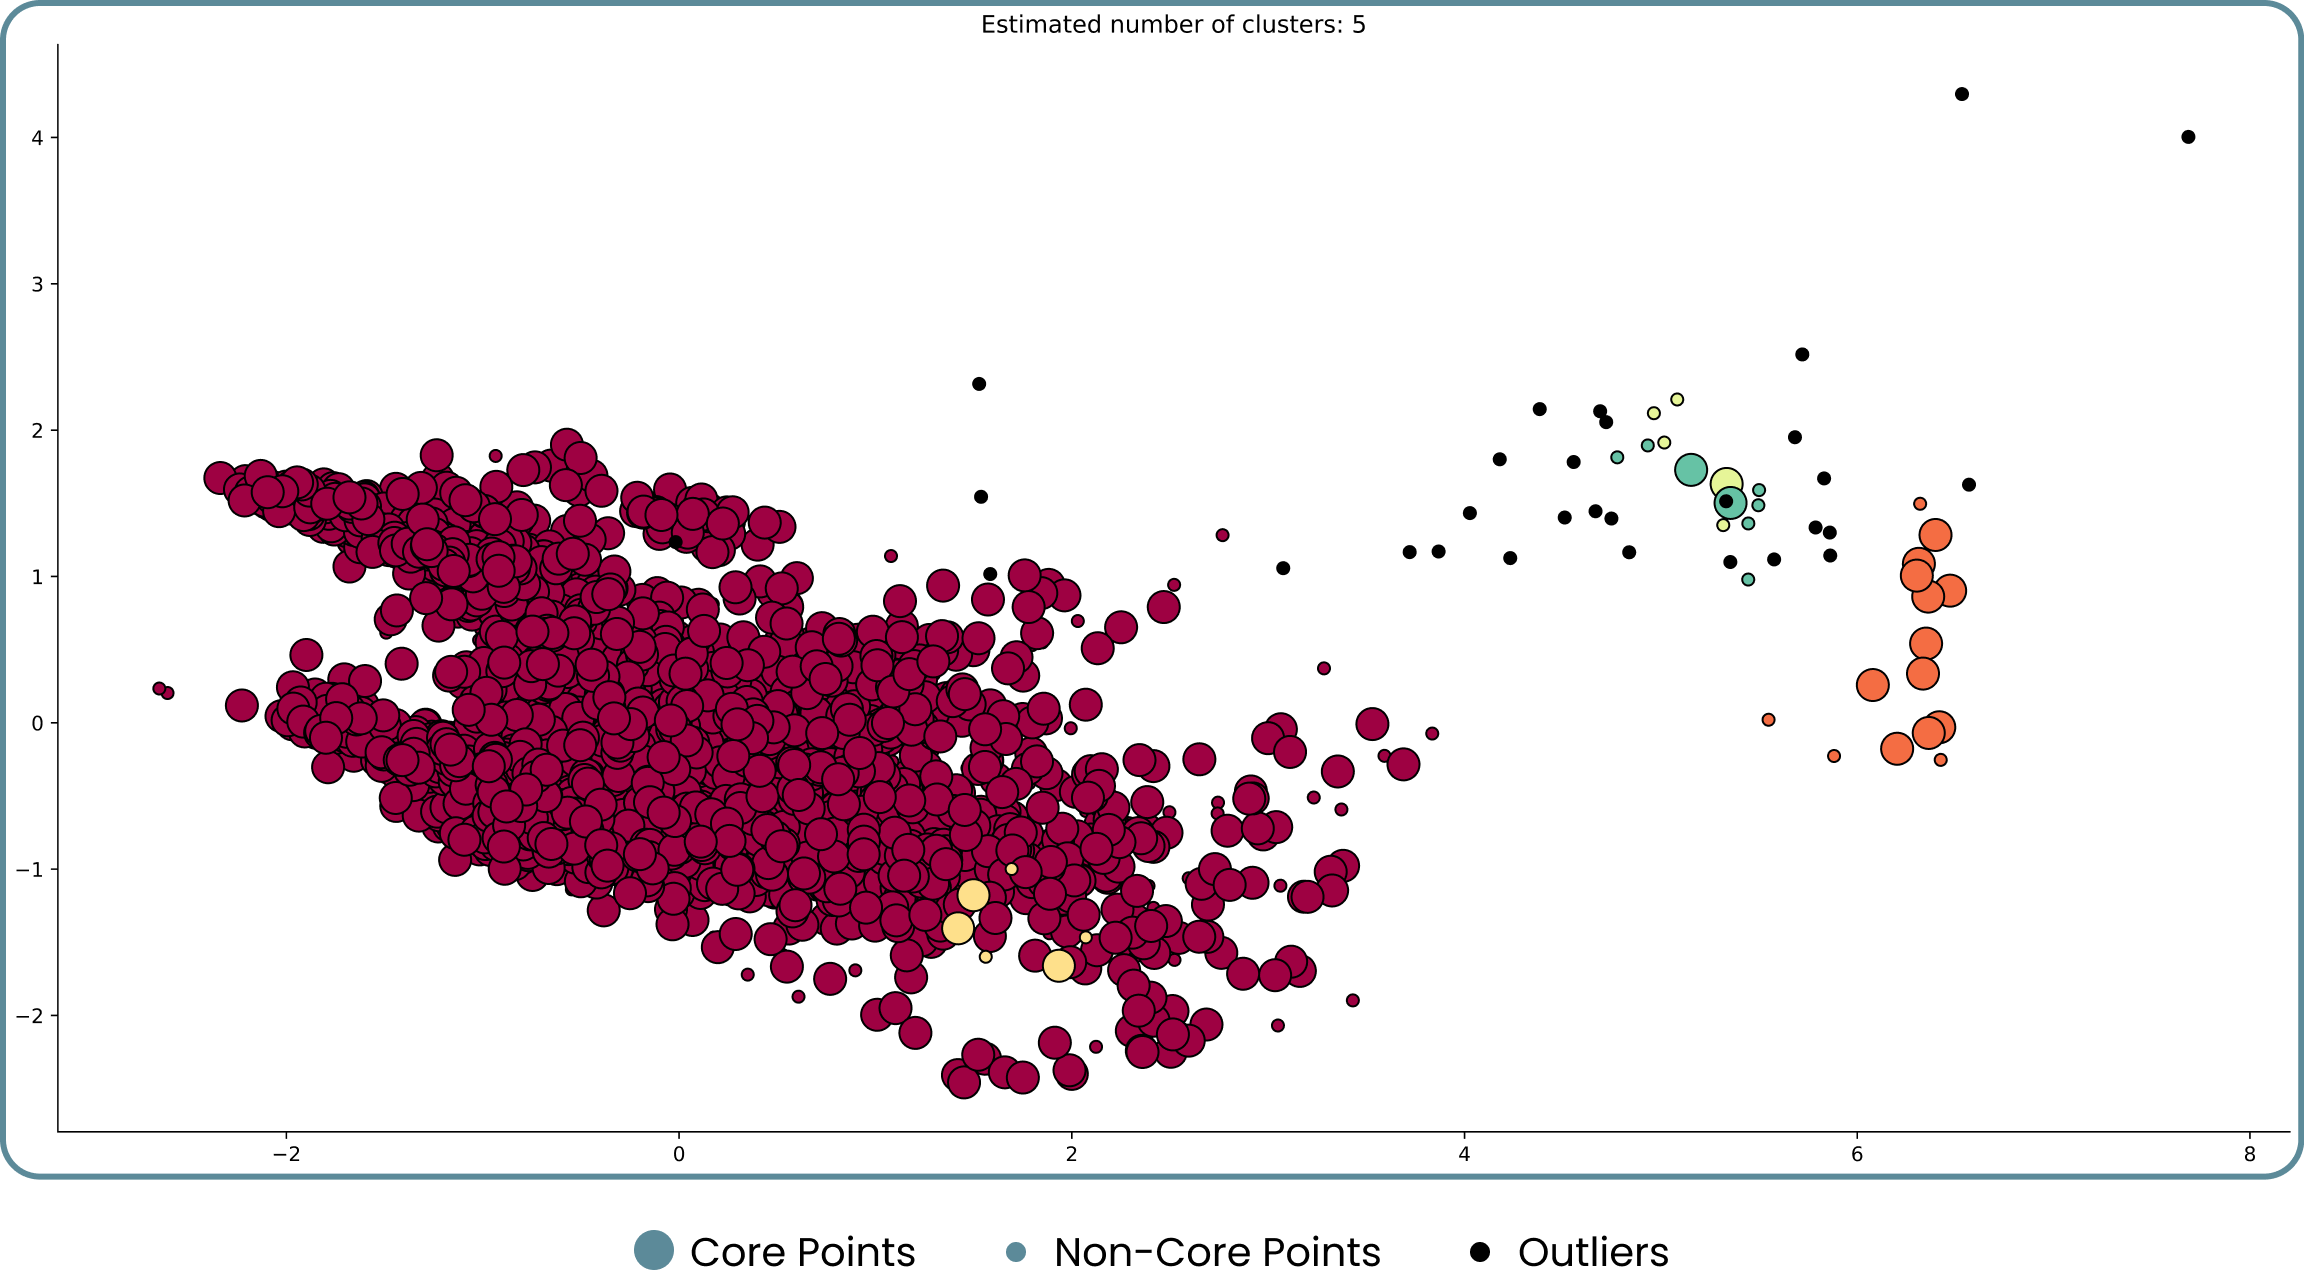
\includegraphics[width=13cm]{Images/3/clusters.png}
    \caption{Graphic representation of clusters in 2 components with PCA}
\end{figure}

Probabilmente, trattandosi di dimensioni fittizie, questa raffigurazione non risulta molto significativa da guardare a occhio nudo, ma fa capire come ha funzionato il DBSCAN. Difatti i diversi colori con cui sono rappresentati i punti rappresentano i diversi cluster generati. Invece la dimensione del punto distingue i core points dai non-core points. Infine, i piccoli pallinni neri rappresentano gli outliers evidenziati dall'algoritmo.

\subsection{Features importance}
\label{sec:testing-importance}

Come descritto nella sezione \ref{sec:importance} uno step fondamentale è stato quello di analizzare le feature importance per ogni modello dopo l'implementazione di DBSCAN grazie alla logistic regression.

\begin{figure}[H]
    \centering
    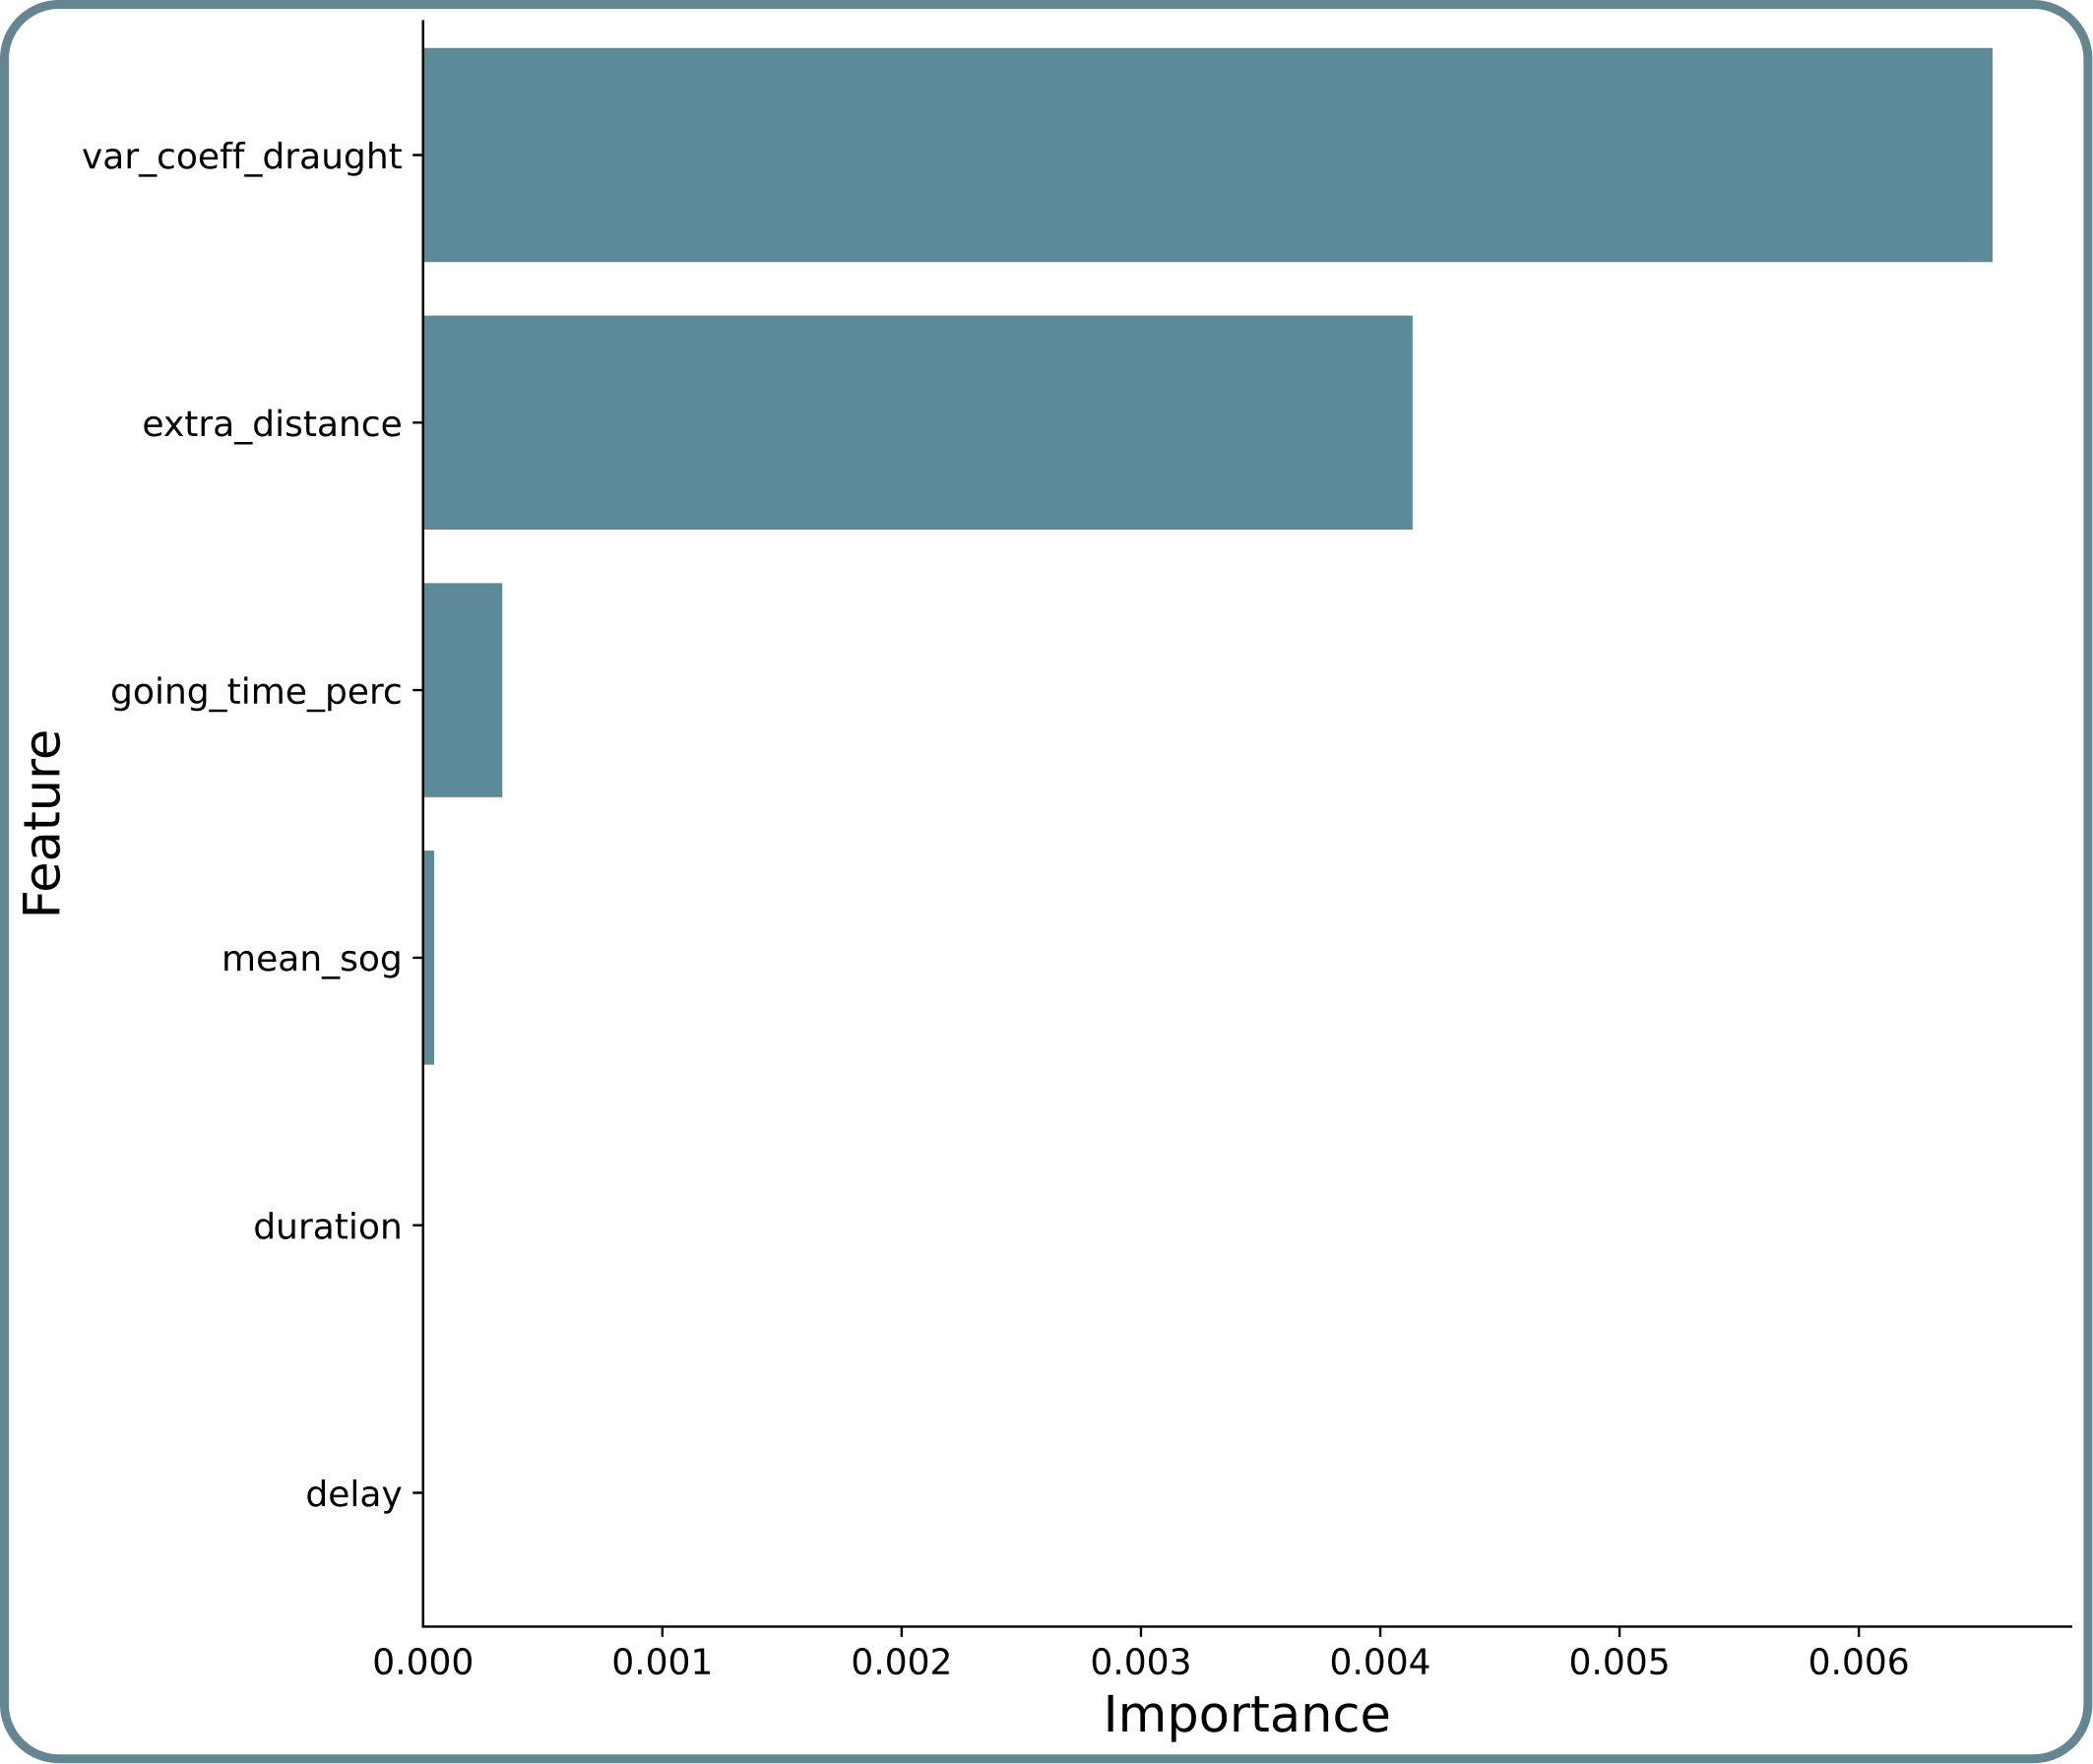
\includegraphics[width=13cm]{Images/3/importance.png}
    \caption{Feature importance classification for Cluster \#1}
\end{figure}

Avendo un grafico come questo per ogni cluster è stato possibile capire nel complesso quali sono le features più importanti al fine della classificazione degli outliers.

\subsection{Anomaly 1 - Extra distance}
\label{sec:anomaly-1}

L'anomalia collegata alla feature \textbf{extra distance} occupa le prime posizioni nella maggior parte delle classifiche di feature importance dei modelli risultanti.

Naturalmente per la valutazione di questa anomalia non sono stati considerati tragitti con punti di terraferma all'interno della via, 

\begin{lstlisting}[language=Python]
extra_distance = ideal_distance - actual_distance
\end{lstlisting}

\begin{itemize}
\item Model Accuracy: \textbf{0.9189} \textcolor{green}{> 0.8}
\item T-test p value: \textbf{3.32e-03} \textcolor{green}{< 0.05}
\item Average Value for outliers: \textbf{196km}
\item Average Value for non outliers: \textbf{67.24km}
\end{itemize}


\begin{figure}[H]
    \centering
    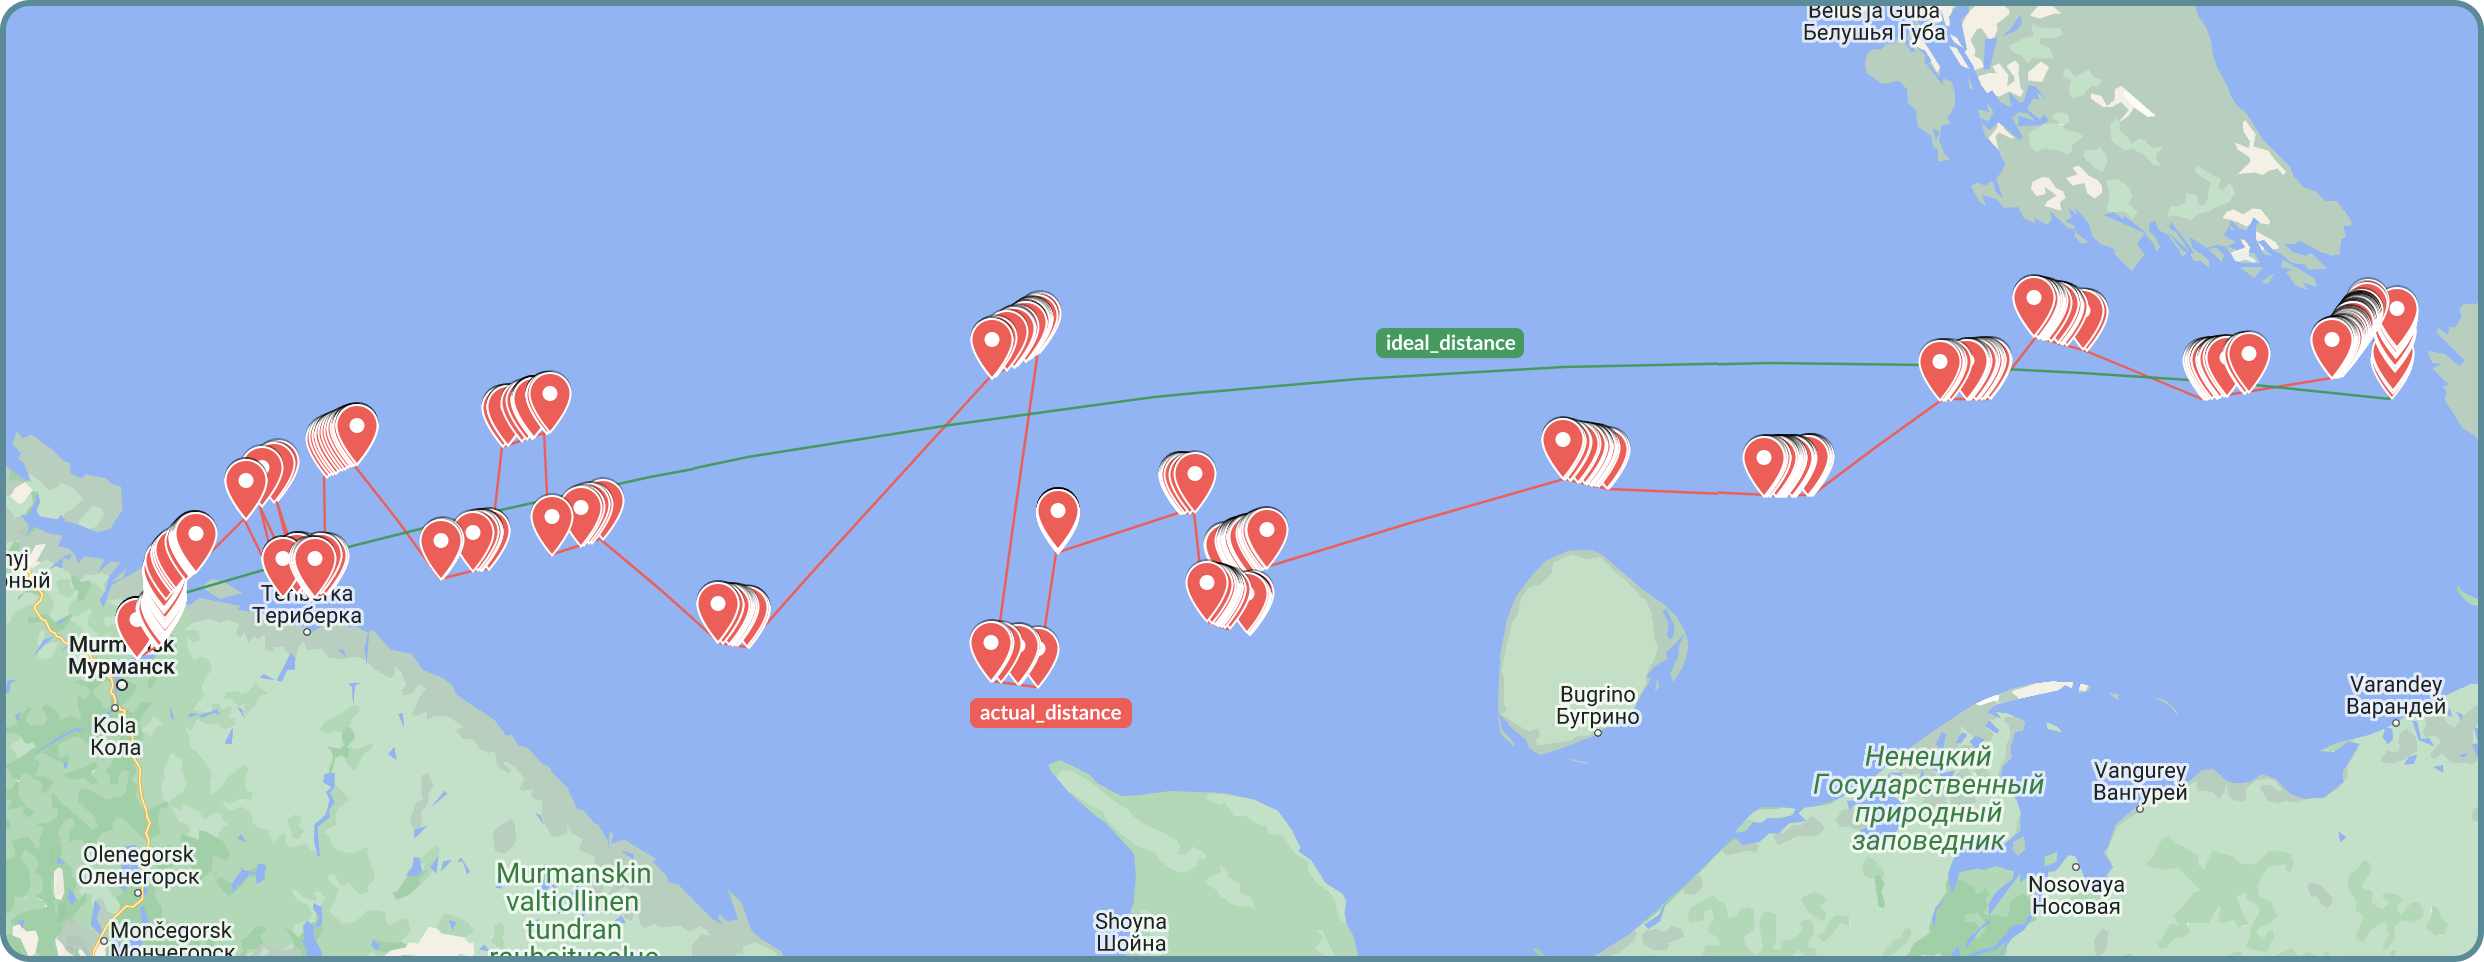
\includegraphics[width=16.5cm]{Images/3/anomaly-1.png}
    \caption{Vessel (MMSI 273397870) with a actual\_distance that differs greatly from the ideal\_distance.}
\end{figure}

\subsection{Anomaly 2 - Draught relative standard deviation}
\label{sec:anomaly-2}

\begin{itemize}
\item Model Accuracy: \textbf{0.9189} \textcolor{green}{> 0.8}
\item T-test p value: \textbf{3.32e-03} \textcolor{green}{< 0.05}
\item Average Value for outliers: \textbf{196km}
\item Average Value for non outliers: \textbf{67.24km}
\end{itemize}

\begin{figure}[H]
    \centering
    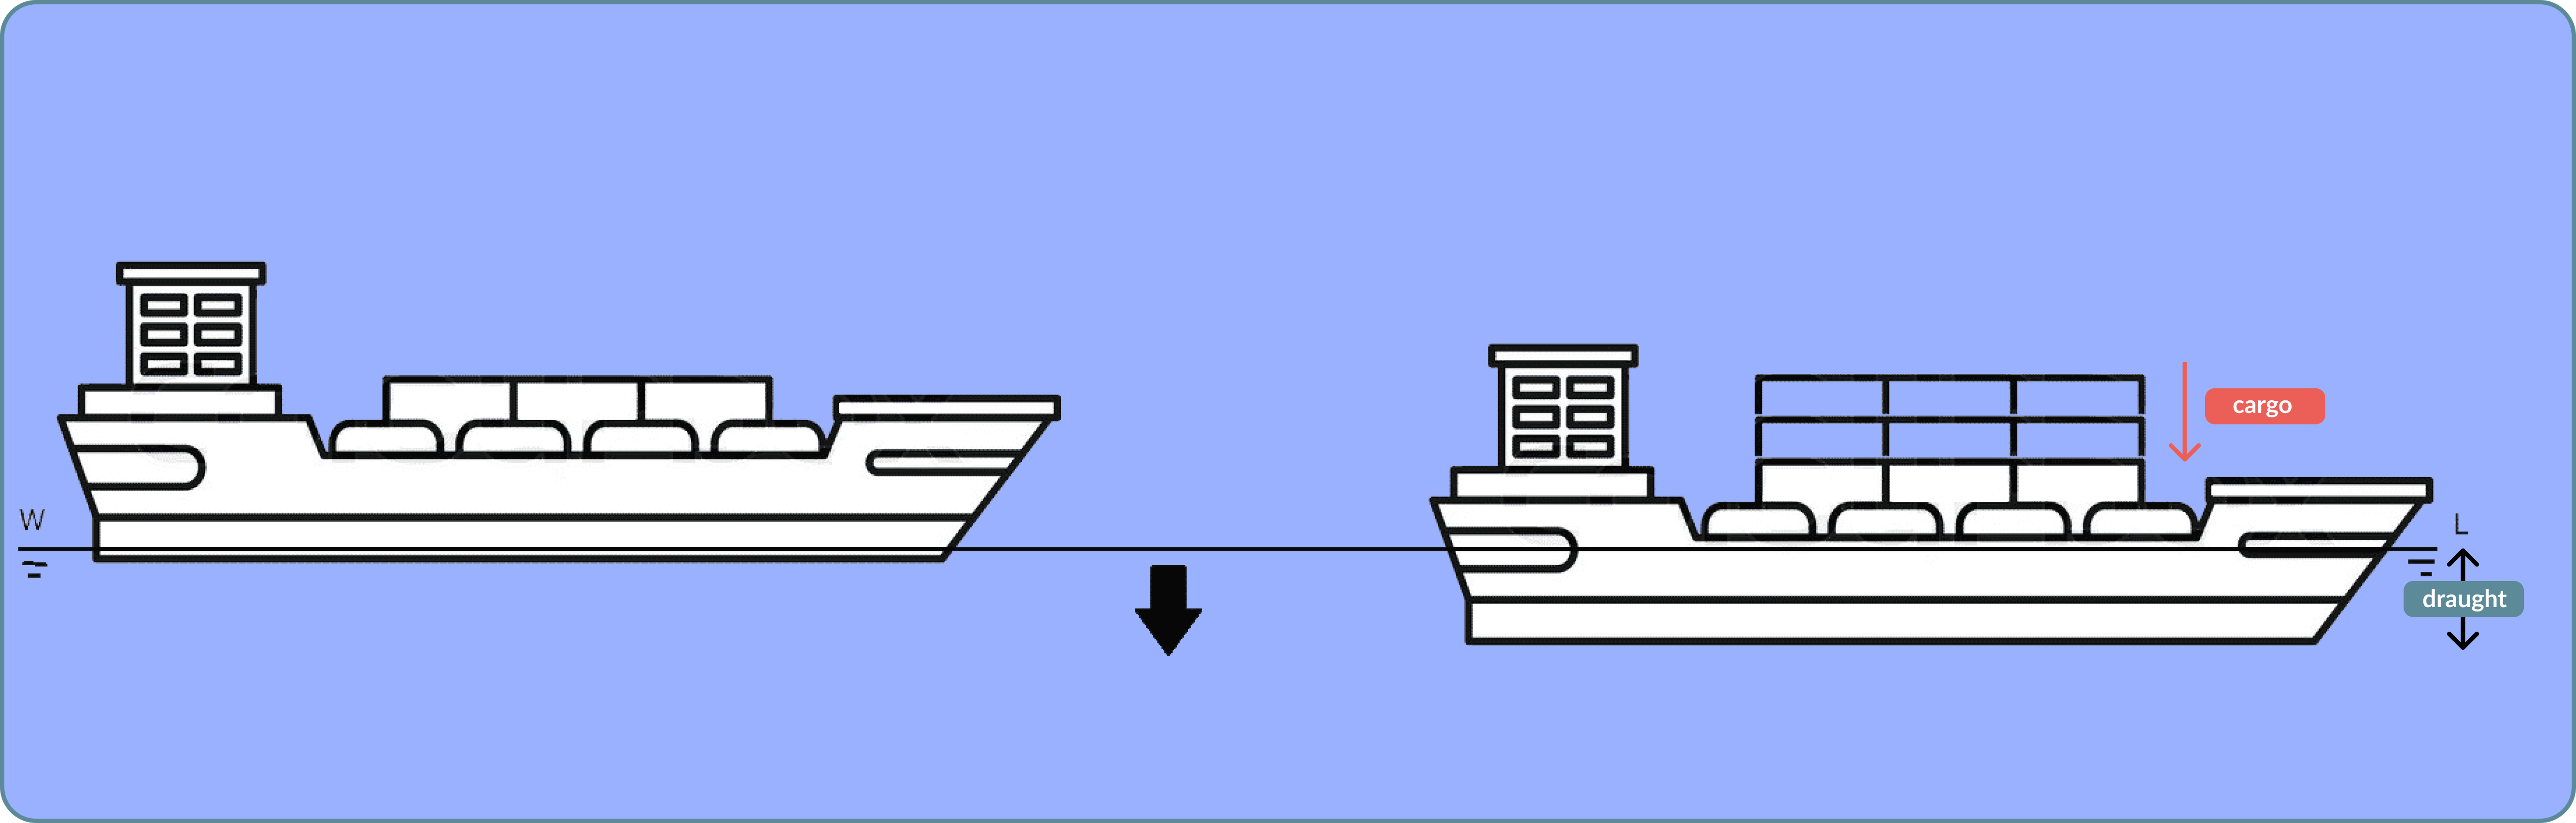
\includegraphics[width=16.5cm]{Images/3/anomaly-2.png}
    \caption{Draught value as proxy of cargo weight.}
\end{figure}

\subsection{Anomaly 3 - Going time percentage}
\label{sec:anomaly-3}

\begin{figure}[H]
    \centering
    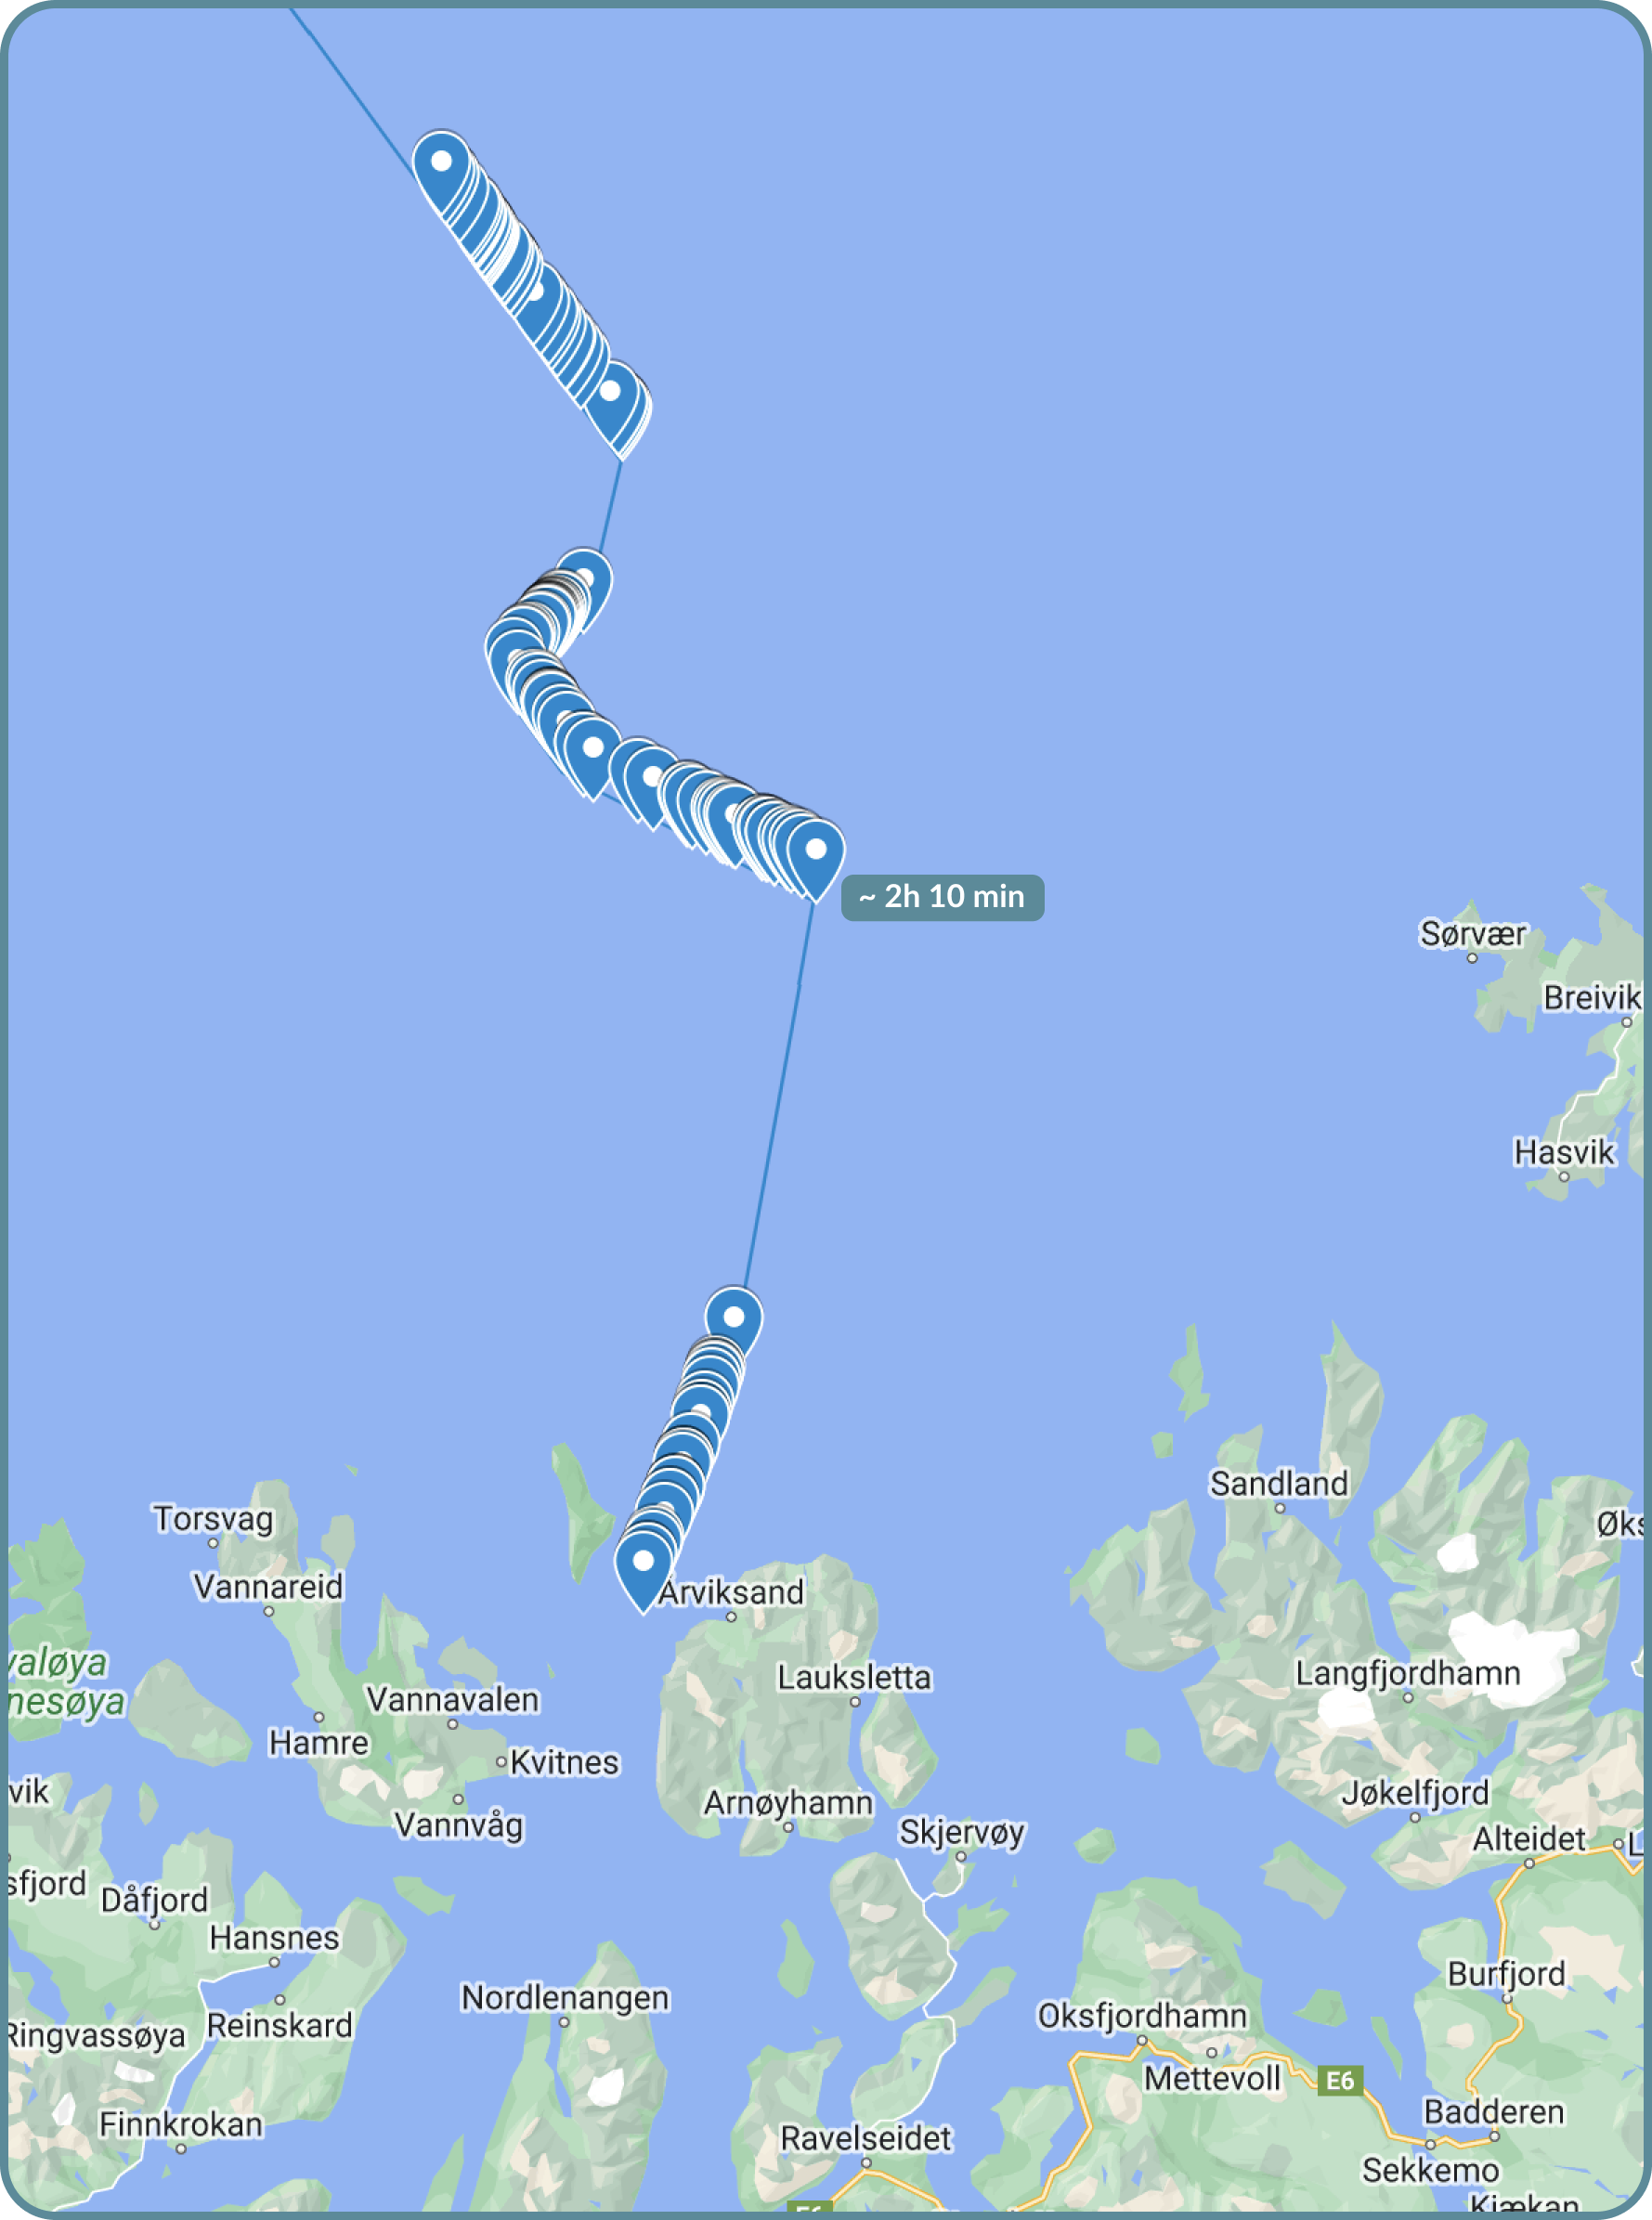
\includegraphics[width=10cm]{Images/3/anomaly-3.png}
    \caption{Vessel (MMSI 273397870) with anomal going time stall point.}
\end{figure}
